%============================================================%
\documentclass[a4paper,12pt]{article}
%%%%%%%%%%%%%%%%%%%%%%%%%%%%%%%%%%%%%%%%%%%%%%%%%%%%%%%%%%%%%%%%%%%%%%%%%%%%%%%%%%%%%%%%%%%%%%%%%%%%%%%%%%%%%%%%%%%%%%%%%%%%%%%%%%%%%%%%%%%%%%%%%%%%%%%%%%%%%%%%%%%%%%%%%%%%%%%%%%%%%%%%%%%%%%%%%%%%%%%%%%%%%%%%%%%%%%%%%%%%%%%%%%%%%%%%%%%%%%%%%%%%%%%%%%%%
\usepackage{eurosym}
\usepackage{vmargin}
\usepackage{amsmath}
\usepackage{graphics}
\usepackage{epsfig}
\usepackage{subfigure}
\usepackage{multicol}
\usepackage{fancyhdr}
\usepackage{listings}
\usepackage{framed}
\usepackage{graphicx}
\usepackage{amsmath}
\usepackage{enumerate}
\usepackage{chngpage}
%\usepackage{bigints}


\setcounter{MaxMatrixCols}{10}

\begin{document}
	\begin{center}
		
\includegraphics[scale=0.55]{images/shieldtransparent2}
	\end{center}
	
	\begin{center}
		\vspace{1cm}
		\large \bf {FACULTY OF SCIENCE AND ENGINEERING} \\[0.5cm]
		\normalsize DEPARTMENT OF MATHEMATICS AND STATISTICS \\[1.25cm]
		\large \bf {END OF SEMESTER EXAMINATION PAPER 2016} \\[1.5cm]
	\end{center}
	
	\begin{tabular}{ll}
		MODULE CODE: MA4605 & SEMESTER: Autumn 2016 \\[1cm]
		MODULE TITLE: Chemometrics & DURATION OF EXAM: 2.5 hours  \\
		 & \\ [1cm]
		LECTURER: Mr. Kevin O'Brien & GRADING SCHEME: 100 marks \\
		& \phantom{GRADING SCHEME:} \footnotesize {60\% of module grade} \\[1cm]
EXTERNAL EXAMINER: Prof. A. Marshall & \\
	\end{tabular}
\vspace{0.3cm}
	\begin{center}
		{\bf INSTRUCTIONS TO CANDIDATES}
	\end{center}
	
	{\noindent \\ Scientific calculators approved by the University of Limerick can be used. \\
		Formula sheet and statistical tables provided at the end of the exam paper.\\
		There are 5 questions in this exam. Students must attempt any 4 questions.}
	%====================================================================== %
	\newpage
\bigskip
%--------------------------------------------------------------------------------------- %

\subsection*{Question 1. (25 marks) Inference Procedures}\label{sec:question-1.-(25-marks)-inference-procedures-and-distributional-testing}
	
\begin{itemize}
	\item[(a)]
 The concentration of nicotine was determined by gas chromatography in each of two samples of known concentrations 10 ng/ml and 50 ng/ml.
\begin{framed}
	\begin{verbatim}
	Data: Sample (Lo): m = 10 ng/ml, n=14.
	
	8.40, 9.59, 9.38, 9.10, 10.78, 11.41, 9.94, 
	10.08, 12.11, 9.10, 9.59, 10.36, 10.41, 10.52.
	
	Data: Sample (Hi): m = 50 ng/ml, n=10.
	
	47.5, 48.4, 48.8, 48.4, 46.8, 
	46.2, 48.6, 50.6, 45.5, 46.1.
	\end{verbatim}
\end{framed}


\noindent The following blocks of \texttt{R} code (i.e. blocks A to E) are based on the data for this assessment. Write a short report on your conclusion for this assessment. 

\begin{itemize}
	\item[(i)] (12 Marks) State the purpose of each code segment and interpret it. Remember to state the null and alternative hypotheses for each segement.
	\item[(ii)] (3 Marks) Provide an overall conlcusion to the analysis.
\end{itemize}




\noindent \textbf{Block A} (2 Marks)
\begin{framed}
\begin{verbatim}
> grubbs.test(Lo)

Grubbs test for one outlier

data:  Hi
G = 2.09700, U = 0.63573, p-value = 0.1561
alternative hypothesis: highest value 12.11 is an outlier


> grubbs.test(Hi)

Grubbs test for one outlier

data:  Hi
G = 1.86510, U = 0.57054, p-value = 0.1985
alternative hypothesis: highest value 50.6 is an outlier
\end{verbatim}
\end{framed}	
\noindent \textbf{Block B} (2 Marks)
	\begin{framed}
		\begin{verbatim}
		> var.test(Hi,Lo)
		F test to compare two variances
		
		data:  Lo and Hi
		F = 0.3945, num df = 13, denom df = 9, p-value = 0.1246
		
		alternative hypothesis: 
				true ratio of variances is not equal to 1
		
		95 percent confidence interval:
		0.1029905 1.3066461
		
		sample estimates:
		ratio of variances 
		0.3945149
		\end{verbatim}
	\end{framed}
	
\noindent \textbf{Block C} (2 Marks)
	\begin{framed}
		\begin{verbatim}
		> shapiro.test(Lo)
		
		Shapiro-Wilk normality test
		
		data:  Lo
		W = 0.9779, p-value = 0.9609
		
		
		> shapiro.test(Hi)
		
		Shapiro-Wilk normality test
		
		data:  Hi
		W = 0.9496, p-value = 0.6634
		\end{verbatim}
	\end{framed}
\newpage
\noindent \textbf{Block D} (3 Marks)
	\begin{framed}
		\begin{verbatim}
		> t.test(Lo,Hi)
		
		Welch Two Sample t-test
		
		data:  Lo and Hi
		t = -67.374, df = 14.016, p-value < 2.2e-16
		
		alternative hypothesis: 
				true difference in means is not equal to 0
		
		95 percent confidence interval:
		-38.83294 -36.43706
		sample estimates:
		mean of x mean of y 
		10.055    47.690 
		\end{verbatim}
	\end{framed}

\noindent \textbf{Block E} (3 Marks)
	\begin{framed}
		\begin{verbatim}
		> t.test(Lo,Hi,var.equal=TRUE)
		
		Two Sample t-test
		
		data:  Lo and Hi
		t = -72.6977, df = 22, p-value < 2.2e-16
		
		alternative hypothesis: 
				true difference in means is not equal to 0
				
		95 percent confidence interval:
		-38.70863 -36.56137
		sample estimates:
		mean of x mean of y 
		10.055    47.690 
		
		\end{verbatim}
	\end{framed}
\newpage	
\item[(b)] (5 Marks)

A test of a specific blood factor has been devised such that, for adults in Western Europe, the test score is normally distributed with mean 100 and standard deviation 10. A clinical research organization is carrying out research on the blood factor levels for individuals with a particular disease, with emphasis on the effects of medication on the blood factor level.

For a group of 10 volunteer patients the following test scores were obtained both prior to, and after the medication.

\begin{center}
\begin{tabular}{|c||c|c|c|c|c|c|c|c|c|c|} \hline 
Patient	& A	& B	& C	& D	& E	& F	& G &	H &	I &	J	\\ \hline  \hline
Before	& 120& 	140	& 112 &	109&	114	& 116 &	99 & 	108 &	109	& 111 \\ \hline 	
After	& 104&	112	& 110 &	107&	101	& 103 &	101	& 102&	103	& 102 \\ \hline 
\end{tabular} 
\end{center}
	


The organization wishes to determine if there is a significant improvement (lessening of the blood factor level) due to the medication.  Using the output, shown below, write a short report discussing your findings. State the null and alternative hypotheses clearly. (You may assume that the case-wise differences are normally distributed.)

\begin{framed}
\begin{verbatim}
> t.test(Before,After,paired=TRUE)

Paired t-test

data:  Before and After
t = 3.3881, df = 9, p-value = 0.008023
alternative hypothesis: 
  true difference in means is not equal to 0
  
95 percent confidence interval:
3.090618 15.509382
sample estimates:
mean of the differences 
9.3 
\end{verbatim}
\end{framed}
\bigskip

\item[(c)] (5 Marks)
The organization wishes to assess the link between the blood factor level and intake of a particular vitamin.  Using the following output, write a short report discussing your findings. State the null and alternative hypotheses clearly.

\textit{(The \texttt{R} output is presented on the next page)}
\newpage

\begin{framed}
\begin{verbatim}
> cor.test(BloodFactor,Vitamin)

Pearson's product-moment correlation

data:  BloodFactor and Vitamin
t = -3.3672, df = 8, p-value = 0.009827

alternative hypothesis: 
	true correlation is not equal to 0
	
95 percent confidence interval:
-0.9414504 -0.2627543
sample estimates:
cor 
-0.7657047 

\end{verbatim}
\end{framed}
\end{itemize}


%--------------------------------------------------------------------------------------------------------%


\subsection*{Question 2. (25 marks) Regression Models }
	% Multiple Linear Regression
\begin{itemize}
	\item[(a)]

Two methods of determing sulphide content exist: ios-selective estrode (ISE) and gravimetry. Experimental results obtained by both methods are expressed in milligrams of sulphide, and are tabulated below.
\begin{center}
	\begin{tabular}{|c|cccccccccc|}
		\hline
		Sample Number&1&2&3&4&5&6&7&8&9&10\\ \hline
		% after \\: \hline or \cline{col1-col2} \cline{col3-col4} ...
		ISE method & 108 & 12& 152 & 3 & 106 & 11 &  128 & 12& 160& 128 \\ \hline
		gravimetry & 105 & 16& 113 & 1 & 108 &  11 & 141 & 161 & 182& 118\\
		\hline
	\end{tabular}
\end{center}
Two simple linear models are fitted to the data. Model 1 uses the gravimetric measurement as an independent variable to predict the ISE measurement. Conversely, Model 2 uses the ISE measurement as an independent variable used to predict the gravimetric measurement.
% The relevant \texttt{R} output is presented below.\\

\medskip
%Method Comparison Studies
\textit{(The \texttt{R} output is presented on the next page)}
\newpage
	\begin{framed}
\noindent \textbf{Model 1}
		\begin{verbatim}
		Call:
		lm(formula = ISE ~ grav)
		...
		Coefficients:
		Estimate Std. Error t value Pr(>|t|)
		(Intercept)  15.1125    28.8487   0.524    0.615
		grav          0.6997     0.2543   2.751    0.025 *
		---
		Signif. codes:  0 ‘***’ 0.001 ‘**’ 0.01 ‘*’ 0.05 ‘.’ 0.1 ‘ ’ 1
		....
		\end{verbatim}
	\end{framed}\smallskip

	\begin{framed}
\noindent \textbf{Model 2}
		\begin{verbatim}
		Call:
		lm(formula = grav ~ ISE)
		..
		Coefficients:
		            Estimate Std. Error t value Pr(>|t|)
		(Intercept)  38.6215    25.8542   1.494    0.174
		ISE           0.6949     0.2526   2.751    0.025 *
		---
		Signif. codes:  0 ‘***’ 0.001 ‘**’ 0.01 ‘*’ 0.05 ‘.’ 0.1 ‘ ’ 1
		....
		\end{verbatim}
	\end{framed}


\begin{enumerate}[(i)]
	\item (3 Marks) Write down the regression equation for both of the fitted models. Briefly comment on the significant of each of the regression estimates.
	\item (3 Marks) Is a simple linear regression model a suitable approach for this type of analysis? Explain why or why not? 
	\item (4 Marks) Discuss an alternative regression approach for this type of analysis, mentioning any disadvantages in using this alternative approach. 
	\item (4 Marks) The Bland-Altman plot is a graphical technique	commonly used for comparing methods of measurement. Explain how to construct and interpret this plot.
\end{enumerate}

%======================================================
\newpage
\item[(b)] The gold content of a concentrated sea-water sample was determined by using
atomic-absorption spectrometry with the method of standard additions.

The results obtained were as follows:

% latex table generated in R 3.3.1 by xtable 1.8-2 package
% Sat Oct 29 21:05:55 2016
%\begin{table}[ht]
%	\centering
%	\begin{tabular}{rrr}
%		\hline
%		Specimen & Gold Addition   & Absorbance\\
%		& (ng/ml)& \\
%		\hline
%		1 & 30.00 & 0.41 \\ 
%		2 & 40.00 & 0.47 \\ 
%		3 & 50.00 & 0.53 \\ 
%		4 & 60.00 & 0.58 \\ 
%		5 & 70.00 & 0.64 \\ 
%		6 & 0.00 & 0.27 \\ 
%		7 & 10.00 & 0.32 \\ 
%		8 & 20.00 & 0.37 \\ 
%		9 & 80.00 & 0.68 \\ 
%		10 & 70.00 & 0.75 \\ 
%		\hline
%	\end{tabular}
%\end{table}

\begin{framed}
	\begin{verbatim}
>	Gold <-c(30,40,50,60,70,0,10,20,80,70)
>	Abso <-c(0.415,0.472,0.528,0.579,0.641,	
			 0.271,0.323,0.369,0.678,0.752)
>
> summary(lm(Abso~Gold))

Call:
lm(formula = Abso ~ Gold)

Residuals:
Min        1Q    Median        3Q       Max 
-0.034662 -0.014833 -0.013924  0.004695  0.096057 

Coefficients:
Estimate Std. Error t value Pr(>|t|)    
(Intercept) 0.2589060  0.0234791   11.03 4.07e-06 ***
Gold        0.0056720  0.0004668   12.15 1.95e-06 ***
---
Signif. codes:  0 ‘***’ 0.001 ‘**’ 0.01 ‘*’ 0.05 ‘.’ 0.1 ‘ ’ 1

Residual standard error: 0.03852 on 8 degrees of freedom
Multiple R-squared:  0.9486,    Adjusted R-squared:  0.9422 
F-statistic: 147.6 on 1 and 8 DF,  p-value: 1.949e-06
\end{verbatim}
\end{framed}
\begin{itemize}
	\item[(i)] (5 Marks) Explain what the method of standard additions is, what it would be used to determine, and how regression analysis can be used as part of this analysis. Support your answer with sketches.
	\textbf{N.B.}  You are not required to perform any calculations for this example
	
 
\end{itemize}
\item[(c)]
In certain circumstances, Robust Regression may be used in preference to Ordinary Least Squares (OLS) Regression when fitting regression models. Answer the following questions relating to Robust Regression. 

\begin{itemize}
	\item[(i)] (1 Mark) Describe what these circumstances might be.
	\item[(ii)] (1 Mark) State one difference between the OLS and Robust regression techniques in terms of computing regression equations.
\\ \textit{(This question is continued on the next page.)}
	\newpage
	\item[(iii)] (2 Marks) Explain the process of Huber Weighting for Residuals, stating the algorithm used to compute weightings.

	\item[(iv)] (2 Marks) Suppose that Huber Weighting, with a tuning constanct of $k=13.45$, was applied to the observations 
	tabulated below. What would be the outcome of the procedure for each case? 
\end{itemize}
\begin{center}
	\begin{tabular}{|c|c|}
		\hline
		Observation & Residual \\ 
		$i$  & $e_i$ \\ \hline
		11 & -9.07 \\ \hline 
%		14 & 14.54 \\ \hline
		18 & 22.91 \\ \hline
	\end{tabular} 
\end{center}

%\item[(c)] Model appraisal and validation are importants steps in the statistical modelling process. Answer the following questions.
%\begin{itemize}
%	\item[(i)] (2 Marks) In the context of regression models, explain what is meant by Heteroscedascity and Homoscedascity. Support your answers with sketches.
%	 
%
%	\item[(ii)] (1 Mark)  Explain how the \emph{Akaike information criterion} would used to compare two models fitted for the same data.
%
%	\item[(iii)] (1 Mark) Explain why the adjusted $R^2$ value may differ in value from the corresponding multiple $R^2$ value for the same fitted model.
%
%	
%	\item[(iv)] (1 Marks) Explain the term ``Influence" in the context of linear regression models. Support your answer with sketches.
%	\item[(v)] (1 Marks) Explain the  term ``Cook's Distance" in the context of linear regression models. 
%
%
%	
%	\item[(vi)] (2 Marks)  The Durbin Watson Test was carried out to test for Autocorrelation. Briefly describe autocorrelation. You may support your answer with sketches.
%	\item[(vii)] (1 Mark) State your conclusion to the following procedure.
%	\begin{framed}
%		\begin{verbatim}
%		> durbinWatsonTest(ModelQ2)
%		lag Autocorrelation D-W Statistic p-value
%		1     -0.08428163      2.143578   0.806
%		Alternative hypothesis: rho != 0
%		\end{verbatim}
%	\end{framed}
%	
%\end{itemize}
\end{itemize}






%=================================================================================%

\subsection*{Question 3. (25 marks) Experimental Design }
\begin{itemize}
	\item [(a)]

Specimens of milk from dairies in four different districts are assayed for their concentrations of the radioactive isotope Strontium-90. 
The results, in picocuries per litre, are shown in the table below.


	\begin{center}
		\begin{tabular}{|c|cccccccc|c|c|}
			\hline  

	 & &&&&&&& & Mean & St. Dev \\  
		District	&  &&&&&&&& $\bar{x}_i$ & $s_{i}$ \\  
		\hline \hline
A&	28.2	&	30.8	&	27.8	&	32.7	&	29.6	&	31.3	&	32.4	&	32.8	&	30.7	&	1.855	\\ \hline
B&	30.3	&	28.5	&	32.4	&	31.6	&	28.6	&	34.6	&	31.6	&	31.2	&	31.1	&	1.874	\\ \hline
C&	32.9	&	30.6	&	33.6	&	37.1	&	32.6	&	36.1	&	35.5	&	34.4	&	34.1	&	1.976	\\ \hline
D&	32.8	&	34.8	&	34	&	31.6	&	34.8	&	35.2	&	36.4	&	39.6	&	34.9	&	2.251	\\ \hline \hline
			Overall & &&&&&&&&	32.7	&	2.660	\\ \hline
		\end{tabular} 
	\end{center}


%\bigskip
%\begin{itemize}
%	\item[(i)] (2 Marks) Showing your workings, compute the \textbf{Between Group Sum of Squares} (\textit{SSbetween}).
%	\item[(ii)] (2 Marks) Showing your workings, compute the \textbf{Within Group Sum of Squares}\\ (\textit{SSwithin}).
%	\item[(iii)] (2 Mark) Showing your workings, compute the \textbf{Total Group Sum of Squares} (\textit{SStotal}).
%	\item[(iv)] (1 Mark) Complete the \textbf{Degrees of Freedom} Column for the ANOVA table below.
%	\item[(iv)] (1 Mark) Complete the \textbf{Mean Square} Column for the ANOVA table below.
%	\item[(iv)] (1 Mark) Complete the \textbf{F} Column (i.e. the column for Test Statistic) for the ANOVA table below.
%\end{itemize}
\bigskip
{

	\begin{center}
		\begin{tabular}{|l||c|c|c|c|}
			\hline \phantom{makespace} & DF & SS & MS & F \\ \hline
			\hline Between & \phantom{make}? \phantom{make} & \phantom{make}? \phantom{make} & ?  &  ?\\ 
			\hline Within & \phantom{make}? \phantom{make} &\phantom{make}? \phantom{make}  &\phantom{make}? \phantom{make} &  \\ \hline
			\hline Total &  \phantom{make}? \phantom{make} &  &\phantom{makespace}  & \phantom{makespace} \\ 
			\hline 
		\end{tabular} 
	\end{center}
}
\bigskip
The following \texttt{R} output has been produced as a result of analysis of these data:

%Experiment=data.frame(Determinations, Analyst)
%Model=aov(Determinations~Analyst)
%summary(Model)

%Analysis of Variance Table
%
%            Df Sum Sq Mean Sq F value  Pr(>F)
%Analyst      5 0.8611 0.17222   4.236 0.00394 **
%Residuals   36 1.4635 0.04065
%---
%Signif. codes:  0 ‘***’ 0.001 ‘**’ 0.01 ‘*’ 0.05 ‘.’ 0.1 ‘ ’ 1


\begin{enumerate}[(i)]
	\item (8 Marks) Complete the ANOVA table in your answer sheet, replacing the ``?" entries with the correct values.
	\item (2 Marks) What hypothesis is being considered by this procedure.
	\item (2 Marks) What is the conclusion following from the above analysis? State the null and alternative hypothesis clearly.
\end{enumerate}


\newpage
\item[(b)] (4 Marks)

The following outputs are Post-Hoc Procedures for the example in part (a). Interpret these outputs.

\begin{framed}
	\begin{verbatim}
	Tukey Pairwise Comparisons 
	
	Grouping Information Using the Tukey Method and 95% Confidence
	
	District  N    Mean  Grouping
	D         8  34.900  A
	C         8  34.100  A
	B         8  31.100    B
	A         8  30.700    B
	
	\end{verbatim}
\end{framed}

	
	\begin{figure}[h!]
\centering
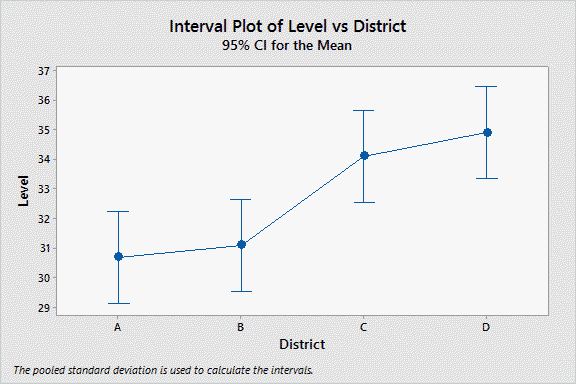
\includegraphics[width=0.85\linewidth]{images/PostHoc1}
\end{figure}
\textit{(The computer output continues on the next page.)}
\newpage
	\begin{figure}[h!]
		\centering

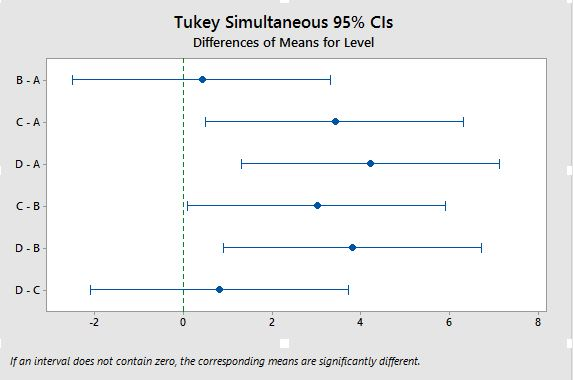
\includegraphics[width=0.85\linewidth]{images/PostHoc4}

\end{figure}

\item[(c)] 
Five standard solutions of chloride were prepared. Four titration methods, each with a different technique of end-point determination, were 
used to analyze each standard solution. The order of the experiments was randomized. The results of chloride found are shown below.


\begin{table}[ht]
	\centering
	\begin{tabular}{|r||c|c|c|c|}
		\hline
		& Method U & Method V & Method W & Method X \\ 
		\hline
	Solution 1 & 10.15 & 10.64 & 10.71 & 10.71 \\ 
	Solution 2 & 10.13 & 10.23 & 10.72 & 10.01 \\ 
	Solution 3 & 10.32 & 10.22 & 10.60 & 10.24 \\ 
	Solution 4 & 10.29 & 10.72 & 10.53 & 10.58 \\ 
	Solution 5 & 9.81 & 10.28 & 10.20 & 9.99 \\ 
		\hline
	\end{tabular}
\end{table}


%\begin{enumerate}[(i)]
%%	\item In the context of the above example, distinguish between the treatment and the blocking variables involved. Give reasons.
%%	
%%	
%%	
%%	\item The above data are an example of a particular experimental design. What is the general name given to this type of experimental design? Name one serious limitation of this type of experimental design.
%%	
%	
%	
%	\item Complete the ANOVA table substituting the symbols ? with their correct values.
%	
%	
%	
%	\item Interpret the results.
%	
%	
%	
%	\item What is the key property of the experimental design above which allows factor effects to be estimated independently of one another. Show how this property presents itself in the above design.
%	
%	
%\end{enumerate}
	
	\noindent You are also given the following information:
	\begin{itemize}
		\item[$\bullet$] $S^2_r = 0.0394$
		\item[$\bullet$] $S^2_c = 0.0305$
		\item[$\bullet$] The variance of concentrations in the table above is $\mbox{Var}(y) = 0.0771$
	\end{itemize}
	\bigskip 
	\noindent The following questions will result in the completion of the ANOVA Table on the next page. The $p-$values for both tests are already provided.
	\begin{itemize}
		\item[(i)](4 Marks) Complete the Sum of Squares column. (Show your workings.)
		\item[(ii)] (1 Mark) State the degrees of freedom for the ANOVA Table.\\ medskip
		
\textit{(This question continues on the next page.)}		
\newpage
		\item[(iii)] (2 Marks) Based on the p-values, provided, what is your conclusion? Clearly state the null and alternative hypotheses for both tests.
	\end{itemize}
	
	\begin{center}
		\begin{tabular}{|c||c|c|c|c|l|}
			\hline Source & DF & SS & MS & F & p-value \\ \hline 
		 Factor A & \phantom{mak} ? \phantom{mak}  & \phantom{mak} ? \phantom{mak}  & \phantom{mak} ? \phantom{mak}  & \phantom{mak} ? \phantom{mak}  &0.0130 * \\ 
			\hline Factor B & \phantom{mak} ? \phantom{mak}  & \phantom{mak} ? \phantom{mak}  & \phantom{mak} ? \phantom{mak}  & \phantom{mak} ? \phantom{mak}  & 0.0196 *    \\ \hline
		Error &  ? & ? & \phantom{mak} ? \phantom{mak}  &  &  \\ 
			\hline \hline Total & ? & ? &  &  &  \\ 
			\hline 
		\end{tabular}
	\end{center} 
\end{itemize}




	

\section*{Question 4. (25 Marks) Experimental Design}
\begin{itemize}
	\item[(a)]
	
	\begin{enumerate}[(i)]
		%-----------------------%
		%\item (2 Marks) What is the purpose of a post hoc test?
		\item (3 Marks) What are the key components that need to be identified when designing an
		experiment?
		
		\item (2 Marks) What is a randomised block design?
		\item (2 Marks) What is an ``a x b" factorial experimental design?
		%	\item (2 Marks)  What is the difference between a between-treatments estimate and a within treatmentsestimate?
		\item (2 Marks) What distinguishes a factorial experiment from a completely randomised experiment or a randomised block experiment?
		
		
	\end{enumerate}


		\item[(b)] 
An experiment is run on an operating chemical process in which the aim is to reduce the
amount of impurity produced. Three continuous variables are thought to affect impurity,
these are agitation speed, concentration of NaOH and temperature. As an initial investigation two settings are selected for each variable these are

\begin{center}
	\begin{tabular}{|c|c|c|}
		\hline
		% after \\: \hline or \cline{col1-col2} \cline{col3-col4} ...
		Factor: &low level & highlevel  \\ \hline
		Agitation speed (rpm) & 15 & 30 \\
		Concentration of NaOH & $40\%$ & $50\%$\\
		
		Temperature ($^{\circ}{\rm F}$) & 150 & 200 \\
		\hline
	\end{tabular}
\end{center}
Readings were recorded of the impurity produced from the chemical process for each combination of the levels of these factors, and each combination was tested twice.
\begin{center}
	\begin{tabular}{|c|c|c|c|c|}
		\hline
		% after \\: \hline or \cline{col1-col2} \cline{col3-col4} ...
		Agitation & Conc NaOH &  Temperature & Impurity & Impurity  \\
		A & C & T & Replicate 1 & Replicate 2  \\ \hline

					-1	&	-1	&	-1	&	45.1	&	44.6	\\ \hline
					
					1	&	-1	&	-1	&	44.9	&	45.3	\\ \hline
					
					-1	&	1	&	-1	&	44.8	&	46.7	\\ \hline
					
					1	&	1	&	-1	&	44.7	&	44.8	\\ \hline
					
					-1	&	-1	&	1	&	33.0	&	35.0	\\ \hline
					
					1	&	-1	&	1	&	53.8	&	51.7	\\ \hline
					
					-1	&	1	&	1	&	32.6	&	33.7	\\ \hline							
					1	&	1	&	1	&	54.2	&	53.2	\\ \hline
				\end{tabular}
			\end{center}
		
\textit{(This question continues on the next page.)}		
\newpage
The data was analysed with statistical computing software, creating the output presented below. Some numbers have been removed.
\begin{framed}
	\begin{verbatim}
	> summary(aov(y~A*C*T, Fact))
	
	Df  Sum Sq Mean Sq  F value    Pr(>F)    
	A            1   .....   .....  405.762  3.85e-08 ***
	C            1     0.1     0.1    0.115    0.7429    
	T            1   .....   .....   12.812    0.0072 ** 
	A:C          1     0.1     0.1    0.083    0.7811    
	A:T          1   .....   .....  437.953  2.85e-08 ***
	C:T          1     0.1     0.1    0.055    0.8200    
	A:C:T        1     2.3     2.3    2.540    0.1497    
	Residuals    8     7.3     0.9                     
	---
	Signif. codes:  0 ‘***’ 0.001 ‘**’ 0.01 ‘*’ 0.05 ‘.’ 0.1 ‘ ’ 1
	
	\end{verbatim}
\end{framed}	
	\begin{itemize}
		\item[(i)] (3 Marks) Calculate the contrasts, the effects and the sum of squares for the main effect A. 
		\item[(ii)] (3 Marks) Calculate the contrasts, the effects and the sum of squares for the interaction effect between A and T.
		\item[(iii)] (3 Marks) Calculate the contrasts, the effects and the sum of squares for the interaction effect between A, C and T.

		\item[(iv)] (3 Marks) Comment on the tests for significant for the main effects and interactions. State your conclusions clearly.
		\item[(v)] (4 Marks) Write down a regression equation that can be used for predicting amounts based on the results of this experiment.
	\end{itemize}
	
\end{itemize}	
%	
%	\begin{center}
%		\begin{tabular}{|c|c|c|c|c|l|}\hline
%			& DF & Sum Sq & Mean Sq & F value&   Pr($>$F)\\  
%			\hline A & $\ldots$ & $\ldots$ & $\ldots$  & $\ldots$ &  0.000979 ***\\ 
%			\hline C & $\ldots$ & $\ldots$ & $\ldots$  & $\ldots$ &  0.934131  \\ 
%			\hline T &\phantom{m} $\ldots$ \phantom{m}  & $\ldots$ & $\ldots$  & $\ldots$ & 0.395554  \\ 
%			\hline A:C & $\ldots$ & $\ldots$ & $\ldots$  & $\ldots$ & 0.944243  \\ 
%			\hline A:T & $\ldots$ & $\ldots$ & $\ldots$  & $\ldots$ & 0.017582 * \\ 
%			\hline C:T & $\ldots$ & $\ldots$ & $\ldots$  & $\ldots$ & 0.072101 \\                 
%			\hline A:C:T & $\ldots$ & $\ldots$ & $\ldots$  & $\ldots$ &  0.028522 *   \\ 
%			\hline Residuals & $\ldots$ & $\ldots$ &  & &  \\ \hline
%			\hline Total & $\ldots$ & 1172.985 &  & &  \\ 	
%			\hline 
%		\end{tabular} 
%	\end{center}
	

	
	

















\section*{Question 5. (25 marks) Statistical Process Control }

\begin{itemize}
	\item[(a)] Answer the following questions on graphical procedures used in Statistical Process Control.\\ \smallskip
	
	\noindent Describe the purpose, the construction and interpretation of each chart or plot. Support your answers with sketches. 
	
	\begin{itemize}

		\item[(i)] (3 Marks) The CUSUM chart.
		\item[(ii)] (3 Marks) The OC chart. 
	\end{itemize}

\textit{(This question continues on the next page.)}		
\newpage	

	\item[(b)] (3 Marks) Write a brief description of the Mahalanobis Distance. Illustrate your answer with a sketch.
	


\item[(c)]
An automobile assembly plant concerned about quality improvement measured sets of five camshafts on twenty occasions throughout the day. The specifications for the process state that the design specification limits are 600$\pm$3mm.


\begin{itemize}
	\item[(i)] (4 Marks) Determine the \emph{Process Capability Indices} $C_p$ and $C_{pk}$, commenting on the respective values. Use the \texttt{R} code output shown below.
	\item[(ii)] (2 Mark)  Explain why there would be a discrepancy between $C_p$ and $C_{pk}$. Illustrate your answer with sketches.
	\item[(iii)] (1 Mark) Comment on the graphical output of the \emph{Process Capability Analysis}, also presented on the next page.
\end{itemize}


\begin{framed}
	\begin{verbatim}
	Process Capability Analysis
	
	Call:
	process.capability(object = obj,  
	spec.limits = c(597, 603))
	Number of obs = 100          Target = 600
	Center = 599.548         LSL = 597
	StdDev = 0.5846948       USL = 603
	
	Capability indices:
  	   Value   2.5%  97.5%
	Cp    ...
	Cp_l  ...
	Cp_u  ...
	Cp_k  ...
	Cpm   1.353  1.134  1.572
	Exp<LSL 0%   Obs<LSL 0%
	\end{verbatim}
\end{framed}



\begin{center}
	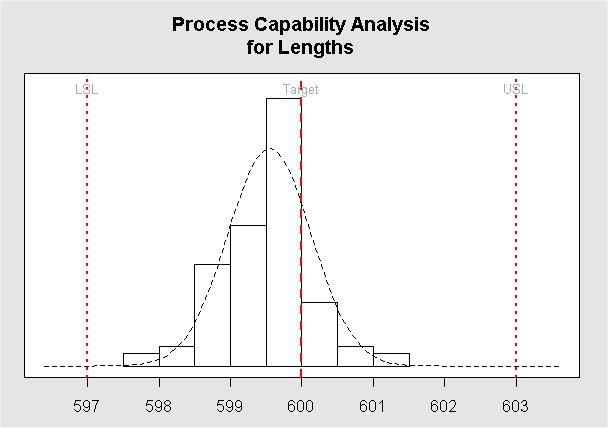
\includegraphics[scale=0.55]{images/ExamQ4hist}
\end{center}

\item[(c)] ($3 \times 3$ Marks) The \textbf{Nelson Rules} are a set of eight decision rules for detecting ``out-of-control" or non-random conditions on control charts. These rules are applied to a control chart on which the magnitude of some variable is plotted against time. The rules are based on the mean value and the standard deviation of the samples.\\

  Discuss any three of these rules, stating their mathematical basis and how they would be used to detect ``out of control" processes. Support your answer with sketch. 


\bigskip 

	\noindent \textit{In your answer, you may make reference to the following properties of the Normal Distribution. Consider the random variable $X$ distributed as
		\[X \sim \mathcal{N}(\mu,\sigma^2)\]
		where $\mu$ is the mean and $\sigma^2$ is the variance of $X$.}
	\begin{itemize}
		\item[$\ast$] $\Pr( \mu - 1\sigma \leq X \leq \mu + 1\sigma ) = 0.6827$
		\item[$\ast$] $\Pr( \mu - 2\sigma \leq X \leq \mu + 2\sigma ) = 0.9545$
		\item[$\ast$] $\Pr( \mu - 3\sigma \leq X \leq \mu + 3\sigma )= 0.9973$
		
	\end{itemize}


\end{itemize}

\newpage


\section*{Formulas and Tables}

\subsection*{Critical Values for Dixon Q Test}


	{
		\Large
		\begin{center}
			\begin{tabular}{|c|c|c|c|}
				\hline  N  & $\alpha=0.10$  & $\alpha=0.05$  & $\alpha=0.01$  \\ \hline
				3  & 0.941 & 0.97  & 0.994 \\ \hline
				4  & 0.765 & 0.829 & 0.926 \\ \hline
				5  & 0.642 & 0.71  & 0.821 \\ \hline
				6  & 0.56  & 0.625 & 0.74  \\ \hline
				7  & 0.507 & 0.568 & 0.68  \\ \hline
				8  & 0.468 & 0.526 & 0.634 \\ \hline
				9  & 0.437 & 0.493 & 0.598 \\ \hline
				10 & 0.412 & 0.466 & 0.568 \\ \hline
				11 & 0.392 & 0.444 & 0.542 \\ \hline
				12 & 0.376 & 0.426 & 0.522 \\ \hline
				13 & 0.361 & 0.41  & 0.503 \\ \hline
				14 & 0.349 & 0.396 & 0.488 \\ \hline
				15 & 0.338 & 0.384 & 0.475 \\ \hline
				16 & 0.329 & 0.374 & 0.463 \\ \hline
			\end{tabular} 
		\end{center}
	}

\subsection*{Two Way ANOVA}
\begin{multicols}{2}
	
\[MS_A = c \times S^2_r\]

\[MS_B = r \times S^2_c\]
\end{multicols}


\subsection*{Control Limits for Control Charts}

\begin{multicols}{2}
	
\[ \bar{\bar{x}} \pm 3\frac{\bar{s}}{c_4\sqrt{n}}\]

\[ \bar{s} \pm 3\frac{c_5\bar{s}}{c_4}\]

\[\left[ \bar{R}D_3, \bar{R}D_4\right]\]
\end{multicols}
\subsection*{$2^3$ Design: Interaction Effects}

\[ AB = \frac{1}{4n} \left[ abc - bc + ab - b - ac + c - a + (1) \right] \]

\[ AC = \frac{1}{4n} \left[ (1) - a + b - ab -c + ac - bc + abc \right] \]

\[ BC = \frac{1}{4n} \left[ (1) + a - b - ab - c - ac + bc + abc \right] \]

\[ABC = \frac{1}{4n} \left[ abc - bc - ac + c - ab + b +  a - (1) \right] \]

\bigskip


\subsection*{Factorial Design: Sums of Squares}

\[\mbox{Effect} =  \frac{\mbox{Contrast}}{4n}\]

\[\mbox{Sums of Squares} =  \frac{\mbox{(Contrast)}^2}{8n}\]

%------------------------------------------------------------------------ %
\normalsize{
\subsection*{Process Capability Indices}
\begin{multicols}{2}
\[ \hat{C}_p = \frac{\mbox{USL} - \mbox{LSL}}{6s}\]

\[ \hat{C}_{pk} = \mbox{min} \left[\frac{\mbox{USL} - \bar{x}}{3s},\frac{\bar{x} - \mbox{LSL}}{3s} \right] \]

\[ \hat{C}_{pm} = \frac{\mbox{USL} - \mbox{LSL}}{6\sqrt{s^2+(\bar{x}-T)^2}}\]
\end{multicols}
	\newpage
	
	%------------------------------------------------------------------------ %
	\Large{
		\subsection*{Factors for Control Charts}
		\begin{tabular}{|c|c|c|c|c|c|c|}
			\hline
			Sample Size (n) 	&	c4 	&	c5 	&	d2 	&	d3 	&	D3 	&	D4	\\	\hline
			2	&	0.7979	&	0.6028	&	1.128	&	0.853	&	0	&	3.267	\\	
			3	&	0.8862	&	0.4633	&	1.693	&	0.888	&	0	&	2.574	\\	
			4	&	0.9213	&	0.3889	&	2.059	&	0.88	&	0	&	2.282	\\	
			5	&	0.9400	&	0.3412	&	2.326	&	0.864	&	0	&	2.114	\\	
			6	&	0.9515	&	0.3076	&	2.534	&	0.848	&	0	&	2.004	\\	
			7	&	0.9594	&	0.282	&	2.704	&	0.833	&	0.076	&	1.924	\\	
			8	&	0.9650	&	0.2622	&	2.847	&	0.82	&	0.136	&	1.864	\\	
			9	&	0.9693	&	0.2459	&	2.970	&	0.808	&	0.184	&	1.816	\\	
			10	&	0.9727	&	0.2321	&	3.078	&	0.797	&	0.223	&	1.777	\\	
			11	&	0.9754	&	0.2204	&	3.173	&	0.787	&	0.256	&	1.744	\\	
			12	&	0.9776	&	0.2105	&	3.258	&	0.778	&	0.283	&	1.717	\\	
			13	&	0.9794	&	0.2019	&	3.336	&	0.770	&	0.307	&	1.693	\\	
			14	&	0.9810	&	0.1940	&	3.407	&	0.763	&	0.328	&	1.672	\\	
			15	&	0.9823	&	0.1873	&	3.472	&	0.756	&	0.347	&	1.653	\\	
			16	&	0.9835	&	0.1809	&	3.532	&	0.750	&	0.363	&	1.637	\\
			17	&	0.9845	&	0.1754	&	3.588	&	0.744	&	0.378	&	1.622	\\
			18	&	0.9854	&	0.1703	&	3.64	&	0.739	&	0.391	&	1.608	\\
			19	&	0.9862	&	0.1656	&	3.689	&	0.734	&	0.403	&	1.597	\\
			20	&	0.9869	&	0.1613	&	3.735	&	0.729	&	0.415	&	1.585	\\
			21	&	0.9876	&	0.1570	&	3.778	&	0.724	&	0.425	&	1.575	\\
			22	&	0.9882	&	0.1532	&	3.819	&	0.720	&	0.434	&	1.566	\\
			23	&	0.9887	&	0.1499	&	3.858	&	0.716	&	0.443	&	1.557	\\
			24	&	0.9892	&	0.1466	&	3.895	&	0.712	&	0.451	&	1.548	\\
			25	&	0.9896	&	0.1438	&	3.931	&	0.708	&	0.459	&	1.541	\\
			\hline
		\end{tabular}
	} % End Large Font
	
\end{document}

Outliers
Boxplots Outliers ( Upper Fence Lower Fence)
Dixon Q-Test
%----------------------------------%
Chi Square 12 Marks
%=====================================================




\end{document}

\section{Question 6- Standby Questions}
\subsubsection*{Part B Regression ANOVA (6 Marks)}
Suppose we have a regression model, described by the following equation
\[ \hat{y} = 28.81 + 6.45x_1 + 7.82 x_2\]
We are given the following pieces of information.
\begin{itemize}
	\item The standard deviation of the response variance $y$ is 10 units.
	\item There are 53 observations.
	\item The \textit{Coefficient of Determination} (also known as the \textit{Multiple R-Squared}) is 0.75.
\end{itemize}
Complete the \textit{Analysis of Variance} Table for a linear regression model.
The required values are indicated by question marks.

\begin{center}
	\begin{tabular}{|c|c|c|c|c|c|} \hline
		\phantom{makespace}	& DF & 	Sum Sq &	Mean Sq &	F value &   	Pr($>$F)    \\ \hline
		Regression &  \phantom{make}?\phantom{make} &	? &	? &	 ? &	$< 2.2e^{-16}$ \\ \hline
		Error  & ? &	? &  	?   &            &       \\ \hline
		Total  & ?  &	? &  \phantom{makespace}	  &   \phantom{makespace}         &    \phantom{makespace}    \\ \hline
	\end{tabular} 
\end{center}
\subsubsection*{Part B - Linear Regression (8 Marks)}
In an experiment to determine hydrolysable tannins in plants by absorption spectroscopy, the following results from ten samples were obtained and are tabulated below. A simple linear regression model, predicting absorbance values using concentration as the independent variable, was fitted to the data. The scatterplot is depicted below.
%%Absorbance= c(0.084, 0.183, 0.326, 0.464, 0.643, 0.707, 0.717, 0.734 ,0.749 ,0.732) ;
%%Concentration= c(0.123, 0.288, 0.562, 0.921, 1.420, 1.717, 1.921, 2.137 ,2.321, 2.467) ;
%%plot(Concentration,Absorbance,pch=18,col="red",font.axis=2,font.lab=2)
%%abline(coef(lm(Absorbance~Concentration)))

%%Conc.Squared = (Concentration^2)
%%Conc.Cubed = (Concentration^3)
%%ModelA = lm(Absorbance~Concentration)
%%ModelB = lm(Absorbance~Concentration+Conc.Squared)
%%ModelC = lm(Absorbance~Concentration+Conc.Squared+Conc.Cubed)
\begin{center}
	\begin{tabular}{|c||c|c|c|c|c|}
		\hline
		%  % after \\: \hline or \cline{col1-col2} \cline{col3-col4} ...
		Sample & 1 & 2 & 3 & 4 & 5 \\ \hline
		Absorbance & 0.084& 0.183& 0.326& 0.464& 0.643\\
		Concentration & 0.123& 0.288& 0.562& 0.921& 1.420\\ \hline
		Sample & 6 & 7 & 8 & 9 & 10 \\ \hline
		Absorbance & 0.707& 0.717& 0.734 &0.749 &0.732\\
		Concentration & 1.717& 1.921& 2.137 &2.321&2.467\\
		\hline
	\end{tabular}
\end{center}
\begin{center}
	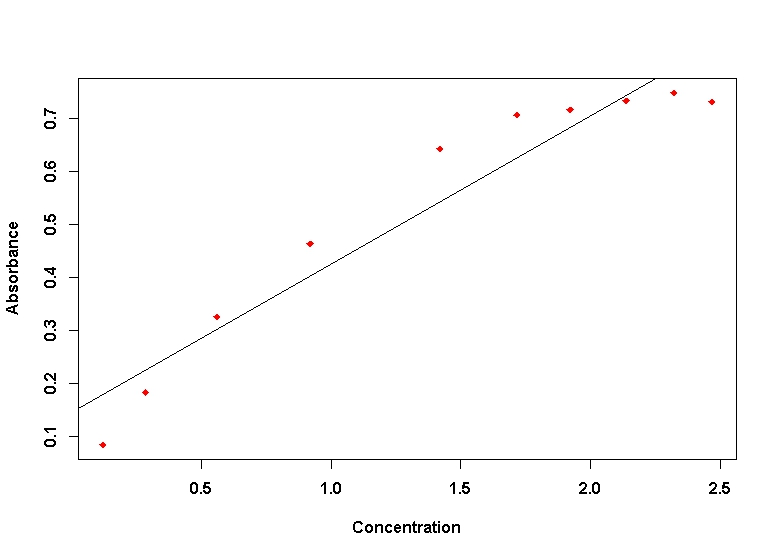
\includegraphics[scale=0.45]{images/ExamQ3plot}
\end{center}
\begin{itemize}
	\item[(i.)] (1 marks) Is the simple linear regression model approach suitable for this study? Explain your answer with reference to the scatter-plot.
	\item[(ii.)] (3 marks) Two polynomial models were also fitted to the data. Description of all three fitted models are found in the three blocks of \texttt{R} code on the following pages. The \emph{Akaike information criterion} is listed, for each of the three fitted models. Write down the regression equations of each of the three models.
	\item[(iii.)] (2 marks) Specify which one of the models you would use. Justify your answer with appropriate statistical values.
	\item[(iv.)] (2 marks) Using the best fitting model, predict a value for absorbance when the concentration level is 1.2 $mg/ml$.
	
\end{itemize}


%
%
%
%\item[(d)] Two polynomial models were also fitted to the data. Description of all three fitted models are found in the three blocks of \texttt{R} code below. The \emph{Akaike information criterion} is also listed, for each of the three fitted models.
%\begin{itemize}
%\item[i.] (4 marks) Write down the regression equation for each of the three linear models.
%\item[ii.] (2 marks) Based on the \emph{Akaike information criterion}, which fitted model can be assumed to be the best fit of the three candidate models.

%\end{itemize}
%\newpage


\begin{framed}
	\noindent \textbf{Model 1}
	\begin{verbatim}
	> summary(Model1)
	Call:
	lm(formula = Absorb ~ Conc)
	...
	Coefficients:
	Estimate Std. Error t value Pr(>|t|)
	(Intercept)    0.14412    0.04721   3.053   0.0158 *
	Concentration  0.28088    0.02930   9.586 1.16e-05 ***
	---
	Signif. codes:  0 ‘***’ 0.001 ‘**’ 0.01 ‘*’ 0.05 ‘.’ 0.1 ‘ ’ 1
	
	Residual standard error: 0.07584 on 8 degrees of freedom
	Multiple R-squared: 0.9199,     Adjusted R-squared: 0.9099
	F-statistic: 91.89 on 1 and 8 DF,  p-value: 1.163e-05
	>
	>
	>AIC(Model1)
	[1] -19.4343
	\end{verbatim}
\end{framed}

\begin{framed}
	\noindent	\textbf{Model 2}
	\begin{verbatim}
	> summary(Model2)
	Call:
	lm(formula = Absorb ~ Conc + Conc.Squared)
	...
	Coefficients:
	Estimate Std. Error t value Pr(>|t|)
	(Intercept)    0.006582   0.008013   0.821    0.439
	Concentration  0.642935   0.015568  41.299 1.27e-09 ***
	Conc.Squared  -0.140573   0.005894 -23.851 5.79e-08 ***
	---
	Signif. codes:  0 ‘***’ 0.001 ‘**’ 0.01 ‘*’ 0.05 ‘.’ 0.1 ‘ ’ 1
	
	Residual standard error: 0.008939 on 7 degrees of freedom
	Multiple R-squared: 0.999,      Adjusted R-squared: 0.9987
	F-statistic:  3592 on 2 and 7 DF,  p-value: 2.879e-11
	>
	>
	> AIC(Model2)
	[1] -61.5338
	\end{verbatim}
\end{framed}


\begin{framed}
	\noindent \textbf{Model 3}
	\begin{verbatim}
	> summary(Model3)
	
	Call:
	lm(formula = Absorb ~ Conc+ Conc.Squared + Conc.Cubed)
	...
	...
	Coefficients:
	Estimate Std. Error t value Pr(>|t|)
	(Intercept)    0.013712   0.011629   1.179   0.2830
	Concentration  0.608682   0.042825  14.213 7.58e-06 ***
	Conc.Squared  -0.108186   0.038088  -2.840   0.0296 *
	Conc.Cubed    -0.008196   0.009518  -0.861   0.4223
	---
	Signif. codes:  0 ‘***’ 0.001 ‘**’ 0.01 ‘*’ 0.05 ‘.’ 0.1 ‘ ’ 1
	
	Residual standard error: 0.009109 on 6 degrees of freedom
	Multiple R-squared: 0.9991,     Adjusted R-squared: 0.9987
	F-statistic:  2306 on 3 and 6 DF,  p-value: 1.422e-09
	>
	>
	> AIC(Model3)
	[1] -60.69903
	\end{verbatim}
\end{framed}
\newpage
%-------------------------------Start of Question 2B%
%\item[(b)](6 marks)
%The scatter-plot contains the regression line for the fitted model. Three diagnostic plots, used to assess the suitability of the fitted model, are presented on the following pages. Provide a brief interpretation for each of the three diagnostic plots described in part(a). The scatter-plot for the data is also presented.

%\begin{center}
%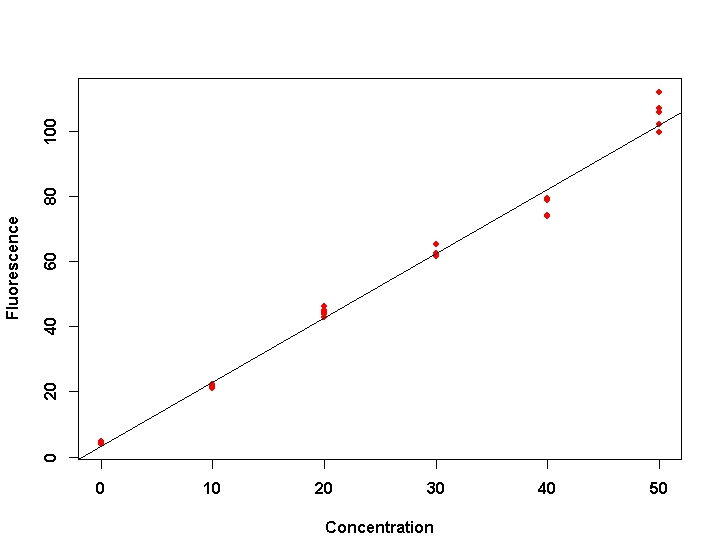
\includegraphics[scale=0.60]{ExamQ2plot2}
%\end{center}
%\newpage
%\begin{center}
%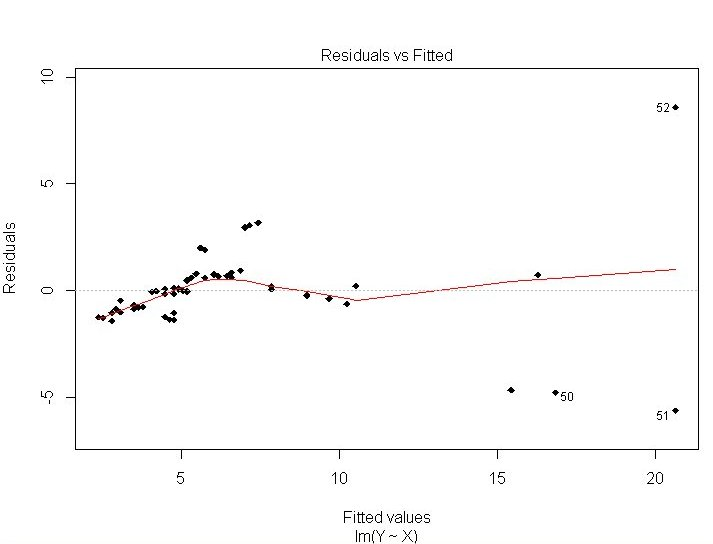
\includegraphics[scale=0.55]{ExamQ2diag1}
%\end{center}
%
%\begin{center}
%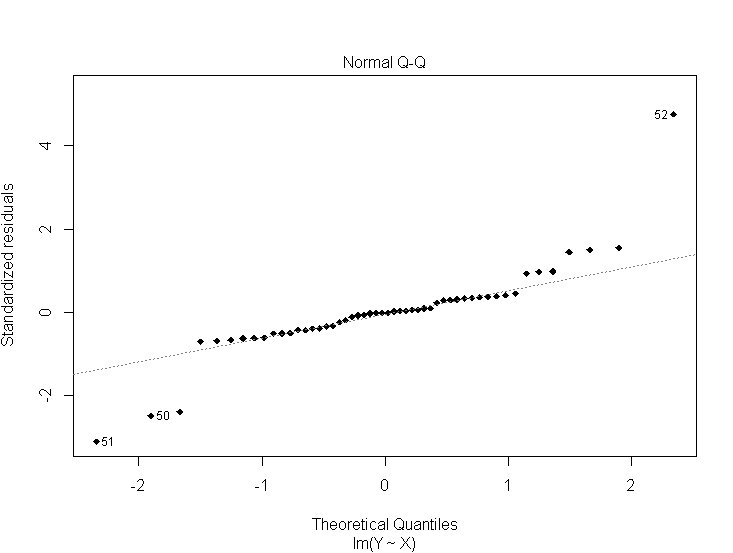
\includegraphics[scale=0.55]{ExamQ2diag2}
%\end{center}
%
%\begin{center}
%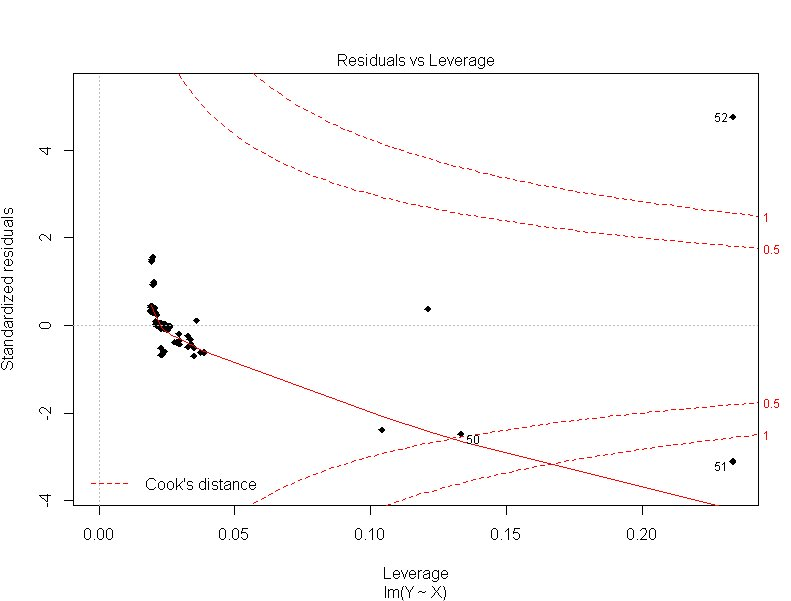
\includegraphics[scale=0.55]{ExamQ2diag3}
%\end{center}



\subsubsection*{Water Nitrate (One Way ANOVA MA4605)}
Four investigators, A, B, C and D, performed six determination of nitrate in water using the same procedure. The results in $\mu$M were:

% Investigator 1 Investigator 2 Investigator 3

\begin{center}
	\begin{tabular}{|c|c|c|c|} \hline
		A  &  B   & C &D\\ \hline \hline
		6.7 & 6.3 & 6.8 & 6.9\\ \hline
		6.8 & 6.2 & 6.9 & 7.1\\ \hline
		6.5 & 6.1 & 7.1 &6.3 \\ \hline
		6.8 & 6.3 & 6.9 &6.2\\ \hline
		6.9 & 6.5 & 7.2 & 6.1\\ \hline
		7.1 & 6.4 & 7.1 & 6.4\\ \hline
	\end{tabular} 
\end{center}



\noindent We are also given the summmary statistics for each of the three investigators, as well as for the samples combined.
\begin{center}
	\begin{tabular}{|c|c|c|}
		\hline  & Sample Mean & Sample Variance \\ 
		\hline A & 6.8 & 0.040 \\ 
		\hline B & 6.3 & 0.020 \\ 
		\hline C & 7 & 0.024 \\ 
		\hline D & 6.5 &  0.164\\
		\hline Overall & 6.65 & 0.1295 \\ 
		\hline 
	\end{tabular} 
\end{center}
\noindent An analysis of variance procedure is used to determine if there is a significant difference between the mean of the determinations made by the three investigators.

% The following output is obtained in R and presented below.

%investigator <- c(6.7, 6.8, 6.5, 6.8, 6.9, 7.1, 6.3, 6.2, 6.1, 6.3, 6.5, 6.4, 
%6.8, 6.9, 7.1, 6.9, 7.2, 7.1)
%A <- investigator[1:6]
%B <- investigator[7:12]
%C <- investigator[13:18]
%
%
%
%group <- factor(rep(1:3,each=6))
%
%aov(investigator~group)
%
%Analysis of Variance Table
%
%Response: investigator

%Df SumSq MeanSq Fvalue Pr(>F)
%
%group ? 1.42333 ? ? 3.133e-05
%
%Residuals 15 ? ?
%
%Total ? 1.9
\smallskip

\noindent The following questions will result in the completion of the ANOVA Table on the next page. The $p-$value is already provided.
\begin{itemize}
	\item[(i.)](3 Marks) Compute the Between Groups Sum of Squares. (Show your workings.)
	\item[(ii.)](3 Marks) Compute the Within Groups Sum of Squares.(Show your workings.)
	\item[(iii.)](2 Marks) Compute the Total Sum of Squares. (Show your workings).
	\item[(iv.)] (1 Mark) State the degrees of freedom for the ANOVA Tables
	\item[(v.)] (1 Mark) Compute the Mean Square values.
	\item[(vi.)] (1 Marks) Compute the test Statistic for this procedure (i.e. the F-value.)
	\item[(vii.)] (3 Marks) This analysis is used to assess if there is any difference between the mean determinations made by the three investigators. What is your conclusion? Clearly state the null and alternative hypothesis.
\end{itemize}
%================================================================================ %
\begin{center}
	\begin{tabular}{|c||c|c|c|c|c|}
		\hline Source & DF & SS & MS & F & p-value \\ \hline 
		\hline Between & \phantom{mak} ? \phantom{mak}  & \phantom{mak} ? \phantom{mak}  & \phantom{mak} ? \phantom{mak}  & \phantom{mak} ? \phantom{mak}  &  $0.000454$ \\ 
		\hline Within &  ? & ? & \phantom{mak} ? \phantom{mak}  &  &  \\ 
		\hline \hline Total & ? & ? &  &  &  \\ 
		\hline 
	\end{tabular}
\end{center} 
%===================================================================================================== %

%\subsubsection*{Question 4 Part B (10 Marks)}
%
%
%
%
%The \texttt{R} code and graphical procedures, below and on the following page, are relevant to checking whether the underlying assumptions are met for the ANOVA model in part (b).
%\begin{itemize}
%	\item[i.] (3 marks) What are the assumptions underlying ANOVA?
%	\item[ii.] (4 marks)  Assess the validity of these assumptions for the ANOVA model in part(b).
%	
%\end{itemize}
%\begin{framed}
%	\begin{verbatim}
%	Shapiro-Wilk normality test
%	
%	data:  Residuals
%	W = 0.9719, p-value = 0.3819
%	\end{verbatim}
%\end{framed}
%\begin{framed}
%	\begin{verbatim}
%	Bartlett test of homogeneity of variances
%	
%	data:  Experiment
%	Bartlett's K-squared = 105.9585, df = 1, p-value < 2.2e-16
%	\end{verbatim}
%\end{framed}
%\begin{center}
%	\includegraphics[scale=0.59]{images/ExamQ5boxplot}
%\end{center}
%\newpage
%%qqnorm(resid(Model),pch=18,col="red",font.lab=2,font.axis=2)
%%qqline(resid(Model))
%\begin{center}
%	\includegraphics[scale=0.55]{images/ExamQ5qqplot}
%\end{center}
%\begin{center}
%	\includegraphics[scale=0.55]{images/ExamQ5resid}
%\end{center}
%-----------------------------------------------------------------%

% End of Question
\newpage
\normalsize{
	

\subsubsection*{Question 3 Part D (12 Marks)}
The mercury level of several tests of sea-water from costal areas was determined by atomic-absorption spectrometry. The results obtained are as follows
\begin{center}
	\begin{tabular}{|c||c|c|c|c|c|c|c|c|c|c|c|} \hline
		Conc &0 &10&20&30&40&50&60&70&80&90&100 \\ \hline 
		Abso &0.321& 0.834& 1.254& 1.773& 2.237& 2.741& 3.196& 3.678& 
		4.217& 4.774& 5.261 \\ \hline
	\end{tabular} 
	
\end{center}


The analysis of the relationship between concentration and absorbance is obtained in R and presented below. 
\begin{framed}
	\begin{verbatim}
	x<-seq(0,100,by=10)
	y<- c(0.321, 0.834, 1.254, 1.773, 2.237, 2.741, 3.196, 3.678, 
	4.217, 4.774, 5.261)
	model<- lm(y~x)
	summary(model)
	
	Call:
	lm(formula = y ~ x)
	
	Coefficients:
	Estimate Std. Error t value Pr(>|t|)    
	(Intercept) 0.2933636  0.0234754   12.50 5.45e-07 
	x           0.0491982  0.0003968  123.98 7.34e-16 
	---
	
	Residual standard error: 0.04162 on 9 degrees of freedom
	Multiple R-squared: 0.9994,     Adjusted R-squared: 0.9993 
	F-statistic: 1.537e+04 on 1 and 9 DF,  p-value: 7.337e-16 
	
	confint(model)
	2.5 %     97.5 %
	(Intercept) 0.24025851 0.34646876
	x           0.04830054 0.05009582
	
	\end{verbatim}
\end{framed}

\begin{itemize}
	\item[(i)] (2 marks)
	Determine and interpret the slope and the intercept of the regression line.
	\item[(ii)]  (2 marks) State the 95\% confidence interval for the slope and the intercept coefficients. Interpret this intervals with respect to any relevant hypothesis tests
	\item[(iii)] (2 marks) Explain in which way is the prediction intervals different from the confidence intervals for fitted values in linear regression?
	\item[(iv)] (2 Marks) The following piece of \texttt{R} code gives us a statistical metric. What is this metric? What is it used for? How should it be interpreted.
	
\end{itemize}
\begin{framed}
	\begin{verbatim}
	> AIC(model)
	[1] -34.93389	
	\end{verbatim}
\end{framed}

%=====================================================



%================================================= %
\subsubsection*{Question 3 Part C (7 Marks)}
Six analysts each made seven determinations of the paracetamol content of the same batch of tablets.
The results are shown below. There are 42 determinations in total. 
%The mean determination for each analysts is also tabulated. \\


%Analyst= structure(c(1L, 2L, 3L, 4L, 5L, 6L, 1L, 2L, 3L, 4L, 5L, 6L, 1L,
%2L, 3L, 4L, 5L, 6L, 1L, 2L, 3L, 4L, 5L, 6L, 1L, 2L, 3L, 4L, 5L,
%6L, 1L, 2L, 3L, 4L, 5L, 6L, 1L, 2L, 3L, 4L, 5L, 6L), .Label = c("A",
%"B", "C", "D", "E", "F"), class = "factor")

%Determinations= c(84.32, 84.24, 84.29, 84.14, 84.5, 84.7, 84.61, 84.13, 84.28,
%84.48, 83.91, 84.36, 84.64, 84, 84.4, 84.27, 84.11, 84.61, 84.62,
%84.02, 84.63, 84.22, 83.99, 84.15, 84.51, 84.25, 84.4, 84.22,
%83.88, 84.17, 84.63, 84.41, 84.68, 84.02, 84.49, 84.11, 84.51,
%84.3, 84.36, 84.33, 84.06, 83.81)

\begin{center}
	\begin{tabular}{|c|ccccccc|}
		\hline
		Analyst	& Content		&		&		&		&		&		&		 \\ \hline
		A	&	84.32	&	84.61	&	84.64	&	84.62	&	84.51	&	84.63	&	84.51	 \\
		B	&	84.24	&	84.13	&	84.00	&	84.02	&	84.25	&	84.41	&	84.30	 \\
		C	&	84.29	&	84.28	&	84.40	&	84.63	&	84.40	&	84.68	&	84.36	 \\
		D	&	84.14	&	84.48	&	84.27	&	84.22	&	84.22	&	84.02	&	84.33	 \\
		E	&	84.50	&	83.91	&	84.11	&	83.99	&	83.88	&	84.49	&	84.06	 \\
		F	&	84.70	&	84.36	&	84.61	&	84.15	&	84.17	&	84.11	&	83.81	 \\
		\hline
	\end{tabular}
\end{center}
\bigskip
The following \texttt{R} output has been produced as a result of analysis of these data:

%Experiment=data.frame(Determinations, Analyst)
%Model=aov(Determinations~Analyst)
%summary(Model)
\begin{framed}
	\begin{verbatim}
	Analysis of Variance Table
	
	Df   Sum Sq   Mean Sq   F value    Pr(>F)
	Analyst        5   0.8611   0.17222     4.236   0.00394 **
	Residuals     36   1.4635   0.04065
	---
	Signif. codes:  0 ‘***’ 0.001 ‘**’ 0.01 ‘*’ 0.05 ‘.’ 0.1 ‘ ’ 1
	\end{verbatim}
\end{framed}

%\subsubsection*{Vegetables (ONE WAY ANOVA 4505)}
%
%(c) The following data give the recovery of bromide from spiked samples of vegetable matter, measured using a gas-liquid chromatographic method. The same amount of bromide was added to each specimen. 
%
%The units for all measurements are  mg g-1
%
%\begin{center}
%	\begin{tabular}{|c|c|c|c|}
%		Tomato: & $\{777 790 759 790 770 758 764\}$ & 774 & 142.6667
%		\\ \hline
%		
%		Cucumber: & $\{782 773 778 765 789 797 782\}$ & 781 &  106\\ \hline
%		
%		Asparagus : & $\{786 783 781 785 789 797 782 \}$& 785 & \\ \hline
%	\end{tabular} 
%\end{center}


%-------------------------------------------------------------------------------
%y<-c(777, 789, 769, 790, 770, 759, 764, 782, 774, 778, 765, 789, 
%797, 782, 785, 783, 782, 785, 787, 791, 782)
%
%
%
%T<-y[1:7];C<-y[8:14];A<-y[15:21];
%mean(T);mean(C);mean(A);
%
%-------------------------------------------------------------------------------
%-------------------------------------------------------------------------------

%
%
%\begin{itemize}
%	\item[(i)](3 Marks) Compute the Between Groups Sum of Squares, \textit{Show your workings}
%	\item[(ii)](3 Marks) Compute the Within Groups Sum of Squares, \textit{Show your workings}
%	\item[(iii)](2 Marks) Compute the Total Sum of Squares,\textit{ show your workings}
%	\item[(iv)] (2 Marks) Degrees of Fredom columns
%	\item[(v)] (1 Marks) Mean Square
%	\item[(vi)] (1 Marks) F test Statistics
%\end{itemize}
%\begin{tabular}{|c|c|c|c|c|c|}
%	\hline Source & DF & SS & MS & F & p-value \\ 
%	\hline Between &  &  &  &  &  \\ 
%	\hline Within &  &  &  &  &  \\ 
%	\hline Total &  &  &  &  &  \\ 
%	\hline 
%\end{tabular} 
%\begin{framed}
%	\begin{verbatim}
%	> bartlett.test(y~group)
%	
%	Bartlett test of homogeneity of variances
%	
%	data:  y by group
%	Bartlett's K-squared = 7.9063, df = 2, p-value = 0.01919
%	
%	\end{verbatim}
%\end{framed}

%====================================================================== %


%Experiment=data.frame(Determinations, Analyst)
%Model=aov(Determinations~Analyst)
%summary(Model)

%Analysis of Variance Table
%
%            Df Sum Sq Mean Sq F value  Pr(>F)
%Analyst      5 0.8611 0.17222   4.236 0.00394 **
%Residuals   36 1.4635 0.04065
%---
%Signif. codes:  0 ‘***’ 0.001 ‘**’ 0.01 ‘*’ 0.05 ‘.’ 0.1 ‘ ’ 1

\begin{center}
	\texttt{
		\begin{tabular}{|cc|c|c|c|c|c|}
			\hline
			% after \\: \hline or \cline{col1-col2} \cline{col3-col4} ...
			&&		&		&		&		&		\\
			Response: Y        	&&	Df  	&	Sum Sq 	&	Mean Sq 	&	F value    	&	$Pr(>F)$    	\\
			&&	\phantom{make}	&		&		&		&		\\\hline \hline
			&&		&	\phantom{make}	&		&		&		\\
			Analyst 	&&	\textbf{?}	&	\textbf{?}	&	\textbf{?}	&	\textbf{?}	&	0.00394 **	\\
			&&		&		&		&		&		\\ \hline
			&&		&		&		&		&		\\
			Residuals	&&	\textbf{?}	&	\textbf{?}	&	0.04065	&	&		\\
			&&		&		&		&		&		\\ \hline
			&&		&		&		&		&		\\
			Total	&&	\textbf{?}	&	2.3246	&		&		&		\\
			&&		&		&		&		&		\\ \hline
		\end{tabular}
	}
\end{center}
\begin{itemize}
	\item[(i.)] (6 Marks) Complete the ANOVA table in your answer sheet, replacing the "?" entries with the correct values.\textit{\\ (You are not required to carry out a hypothesis test.)}
	%	\item[ii.] (2 marks) What hypothesis is being considered by this procedure.
	
\end{itemize}
\newpage


\subsubsection*{Question 3 Part B (4 Marks) - check ANOVA Assumptions}
The \texttt{R} code and graphical procedures, below and on the following page, are relevant to checking whether the underlying assumptions are met for an ANOVA model.
\begin{itemize}
	\item[(i.)] (2 marks) State two testable assumptions required for ANOVA procedures? (You may refer to the code output below.)
	\item[(ii.)] (2 marks)  Assess the validity of these assumptions for an ANOVA model based on the following code outputs.
	
\end{itemize}
{
	\normalsize
	\begin{framed}
		\begin{verbatim}
		> #Shapiro-Wilk normality test
		> shapiro.test(resid(model))
		
		Shapiro-Wilk normality test
		
		data:  resid(model)
		W = 0.96108, p-value = 0.4604
		
		\end{verbatim}
	\end{framed}
	\begin{framed}
		\begin{verbatim}
		> bartlett.test(investigator~group)
		
		Bartlett test of homogeneity of variances
		
		data:  investigator by group
		Bartlett's K-squared = 7.1354, df = 3, p-value = 0.0677
		
		\end{verbatim}
	\end{framed}
}
% \begin{center}
% 	\includegraphics[scale=0.59]{image/ExamQ5boxplot}
% \end{center}
% \newpage
% %qqnorm(resid(Model),pch=18,col="red",font.lab=2,font.axis=2)
% %qqline(resid(Model))
% \begin{center}
% 	\includegraphics[scale=0.55]{image/ExamQ5qqplot}
% \end{center}
% \begin{center}
% 	\includegraphics[scale=0.55]{image/ExamQ5resid}
% \end{center}
}
\newpage


\subsection*{Part C Battery - Partial Completion ANOVA (MA4605)}

An engineer is designing a battery for use in a device that will be subjected to some extreme variations in temperature. 

The only design parameter that he can select at this point is the plate material for the battery, and he has three possible choices. 
When the device is manufactured and is shipped to the field, the engineer has no control over the temperature extremes that the device will encounter, and he knows from experience  that temperature will probably affect the effective battery life. 

However, temperature can be controlled in the product development laboratory for the purposes of a test.  The engineer decides to test all three place materials at three temperature levels – 15, 70, and 125 degrees. 

Four batteries are tested at each combination of plate material and temperature, and all 36 tests are run in random order.


The following partial ANOVA table resulted:

Analysis of Variance for Battery Life Data
%----------------------------------------------
\begin{center}
	\begin{tabular}{|l|c|c|c|}\hline
		Source of & Sum of &\phantom{mak} Degrees of \phantom{mak}& Mean \\
		
		Variation & Squares & Freedom  & Square\\
		
		Material types & 2&  10,683.72 & \phantom{mak} 5,341.86\phantom{mak} \\
		
		Temperature & 2& 39,118.72 & 19,559.36\\
		
		Interaction & 4& 9,613.78 & 2,403.44\\
		
		Error &\phantom{mak} 27\phantom{mak}& 18,230.75 & 675.21\\
		
		Total &35&77,646.97 & \\\hline
	\end{tabular} 
\end{center}
% ----------------------------------------------
\begin{itemize}
	\item[(i.)] Carry out appropriate tests stating clearly the null hypotheses and conclusions. 
	
	\item[(ii.)] Would the engineer be satisfied with his design of the experiment? Explain your answer. 
\end{itemize}





\subsubsection*{Question 2 Part C (7 Marks)}
The \texttt{R} code and graphical procedures, below and on the following page, are relevant to checking whether the underlying assumptions are met for the ANOVA model in part (b).
\begin{itemize}
	\item[(i.)] (3 marks) What are the assumptions underlying ANOVA?
	\item[(ii.)] (4 marks)  Assess the validity of these assumptions for the ANOVA model in Part B.
	
\end{itemize}
\begin{framed}
	\begin{verbatim}
	Shapiro-Wilk normality test
	
	data:  Residuals
	W = 0.9719, p-value = 0.3819
	\end{verbatim}
\end{framed}
\begin{framed}
	\begin{verbatim}
	Bartlett test of homogeneity of variances
	
	data:  Experiment
	Bartlett's K-squared = 105.9585, df = 1, p-value < 2.2e-16
	\end{verbatim}
\end{framed}
\begin{center}
	\includegraphics[scale=0.59]{images/ExamQ5boxplot}
\end{center}
\newpage
%qqnorm(resid(Model),pch=18,col="red",font.lab=2,font.axis=2)
%qqline(resid(Model))
\begin{center}
	\includegraphics[scale=0.55]{images/ExamQ5qqplot}
\end{center}
\begin{center}
	\includegraphics[scale=0.55]{images/ExamQ5resid}
\end{center}%
%====================================================================== %

%
%
%\begin{itemize}
%	\item[(i)](3 Marks) Compute the Between Groups Sum of Squares, \textit{Show your workings}
%	\item[(ii)](3 Marks) Compute the Within Groups Sum of Squares, \textit{Show your workings}
%	\item[(iii)](2 Marks) Compute the Total Sum of Squares,\textit{ show your workings}
%	\item[(iv)] (2 Marks) Degrees of Fredom columns
%	\item[(v)] (1 Marks) Mean Square
%	\item[(vi)] (1 Marks) F test Statistics
%\end{itemize}
%\begin{tabular}{|c|c|c|c|c|c|}
%	\hline Source & DF & SS & MS & F & p-value \\ 
%	\hline Between &  &  &  &  &  \\ 
%	\hline Within &  &  &  &  &  \\ 
%	\hline Total &  &  &  &  &  \\ 
%	\hline 
%\end{tabular} 
%\begin{framed}
%	\begin{verbatim}
%	> bartlett.test(y~group)
%	
%	Bartlett test of homogeneity of variances
%	
%	data:  y by group
%	Bartlett's K-squared = 7.9063, df = 2, p-value = 0.01919
%	
%	\end{verbatim}
%\end{framed}

%====================================================================== %
\newpage

\newpage
\section{R Code for Part 3}
\begin{verbatim}
ALL <- c(84.32, 84.51, 84.63, 84.61, 84.64, 84.51, 84.62, 84.24, 84.25, 
84.41, 84.13, 84, 84.3, 84.02, 84.29, 84.4, 84.68, 84.28, 84.4, 
84.36, 84.63, 84.14, 84.22, 84.02, 84.48, 84.27, 84.33, 84.22, 
84.5, 83.88, 84.49, 83.91, 84.11, 84.06, 83.99, 84.7, 84.17, 
84.11, 84.36, 84.61, 83.81, 84.15)

\end{verbatim}
%==================================================%
library(xtable)

nu1 <- 2:10
nu2 <- c(5:15,18,21,24,27,30)

L1 <- length(nu1)
L2 <- length(nu2)
CVs <- matrix(ncol=L1,nrow=L2)


for( i in 1:L2){
	for( j in 1:L1){ 
		CVs[i,j] <- round( qf(0.95,i,j),3)
	}
	
}

colnames(CVs)<- nu1

rownames(CVs)<- nu2

xtable(CVs) 

%======================================================================= %
Dixon

chi Square

Normal

One Way ANOVA

Two Way ANOVA interactions

Test Normality

SPC definitions





min=23
max=89
range=65
gap=31
TS =31/65 = 0.47692
CV =0.396 (5\%)
Reject Ho


